\documentclass{article}
\usepackage[utf8]{inputenc}

\title{Tarea 2 de Metodos Computacionales}
\author{Christian David Forero Pulido}
\date{19 / 07 / 2019}

\usepackage{natbib}
\usepackage{graphicx}
\usepackage{mathrsfs,amsmath}
\usepackage{graphicx}
\usepackage{subcaption}
\usepackage{epstopdf}
\usepackage{float}
\usepackage{authblk}
\usepackage{amsmath}
\usepackage{amssymb}
\usepackage{listings}

\DeclareUnicodeCharacter{2212}{-}
\begin{document}

\maketitle

\section*{Introduction}

Este proyecto consta dos partes, la primera es usar transformadas de fourier para generar imagenes hibridas y la segunda es comparar tres metodos para resolver ecuaciones diferenciales.

\section{Imagenes Hibridas}
las imagenes que se van a fusionar por el metodo de imagenes hibridas son las figuras \ref{fig:mesh1} y \ref{fig:mesh2}, cara triste y feliz respectivamente.
\\
\begin{figure}
    \centering
    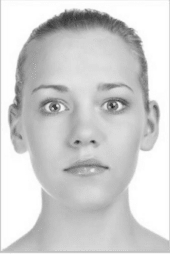
\includegraphics{cara_02_grisesMF.png}
    \caption{Cara triste}
    \label{fig:mesh1}
\end{figure}

\begin{figure}
    \centering
    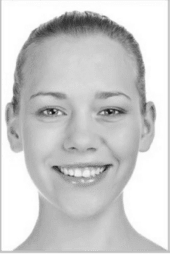
\includegraphics{cara_03_grisesMF.png}
    \caption{Cara feliz}
    \label{fig:mesh2}
\end{figure}

Las imagenes hibridas se basan en hacer un filtro de fourier, y pasar una imagen con filtro de frecuencias bajas y otra imagen con un filtro de frecuencias altas. Posteriormente se suman las transformadas de fourier y despues de hacen las transformadas inversas de fourier, obteniendo las imagenes hibridas. Las transformadas de fourier de ambas imagenes son \ref{fig:mesh3}, donde la cara triste el la de la izquierda y la cara feliz es la de la derecha. 
\\
\begin{figure}
    \centering
    \includegraphics{FFtIm.pdf}
    \caption{Transformadas de Fourier de las imagenes}
    \label{fig:mesh3}
\end{figure}

\begin{figure}
    \centering
    \includegraphics{ImProceso.pdf}
    \caption{Transformadas Fourier filtradas}
    \label{fig:mesh4}
\end{figure}

Estas imagenes funcionan de tal manera que la imagen \ref{fig:mesh1} que se pasa por filtro de baja frecuencia, es decir que solo se mantienen las frecuencias menores a cierto valor $t$, y se ve dicha imagen cuando se acerca la imagen hibrida(esto por ser las frecuencias bajas). Mientras que la imagen \ref{fig:mesh2} que se pasa por un filtro de frecuencias altas, es decir que solo se mantienen las frecuencias mayor a un valor $t$, se ve cuando se aleja la imagen hibrida (esto por ser las frecuencias altas). La transformada de fourier filtrada puede apreciarse en la figura \ref{fig:mesh4}, donde la cara triste es la imagen de la izquierda y la cara feliz es la imagen de la derecha.El valor de elegido para la imagen hibrida fue de $t=22$, donde las unidades estan normalizadas respecto a la transformada de furier de toda la imagen, y el resultado se aprecia en la figura \ref{fig:mesh5}.

\begin{figure}
    \centering
    \includegraphics{ImHybrid.pdf}
    \caption{Imagen hibrida}
    \label{fig:mesh5}
\end{figure}

\section{Solucion a Ecuaciones Diferenciales de Segundo Orden}

Para este punto del proyecto, se van a usar tres metodosm para la solucion de la ecuacion diferencial:
\begin{equation}
    \frac{d^2 \vec{x}}{dt^2} = - GM_{sol} \frac{\vec{r}}{r^3}
\end{equation}

Los metodos que se van a comparar para tres $dt$ diferentes son el metodos de Euler, LeapFrog y RungeKutta. Para solucionar esta ecuacion diferencial solo se tuvieron en cuenta las cordenadas $x$ y $y$, y se usaron las condiciones iniciales  $x = 0.1163$ UA, $y = 0.9772$ UA, $Vx = −6.35$ UA/anios y $Vy = 0.606$ UA/anios adicionalmente cabe aclaran que todo esta en unidades de masas solares, $AU$ y $anios$
\\
Se usaron $dt = 0.05$, $dt = 0.01$ y $dt = 0.001$, se graficaron las
posiciones de $x$ contra $y$, las velocidades $v_{x}$ contra $v_{y}$, la energia contra el tiempo y el momento angular contra el tiempo.
\\
La formula usada para encotrar la energia fue:
\begin{equation}
    E = \frac{1}{2} M_{tierra} (v_{x}^2 v_{y}^2)
\end{equation}
La formula usada para encontrar el momento fue:
\begin{equation}
    L = M_{tierra}(v_{x} y - v_{y} x)
\end{equation}

Finalmente los resultados de la posicion fueron los mostrados en la figura \ref{fig:mesh6}, como podemos apreciar el metodo de euler fue el peory runge kutta fue el mejor, sin embargo todos los metodos mejoraron considerablemente cuando se disminuyo el $dt$.

\begin{figure}
    \centering
    \includegraphics[width=\textwidth]{XY_met_dt.pdf}
    \caption{Posicion durante 20 anios de la tierra}
    \label{fig:mesh6}
\end{figure}

Similarmente con las posiciones, la velocidades que son mostradas en la figura \ref{fig:mesh7} el metodo de euler fue el peory runge kutta fue el mejor, sin embargo todos los metodos mejoraron considerablemente cuando se disminuyo el $dt$.

\begin{figure}
    \centering
    \includegraphics[width=\textwidth]{VxVy_met_dt.pdf}
    \caption{Velocidad durante 20 anios de la tierra}
    \label{fig:mesh7}
\end{figure}

Por ultimo al ver las graficas de energia (figura \ref{fig:mesh8}) y las graficas de momento (figura \ref{fig:mesh9}), podemos concluir que el mejor metodo es runge kutta, seguido por leap frog, pues sucede lo mismo que con las posiciones y las velocidades.

\begin{figure}
    \centering
    \includegraphics[width=\textwidth]{Ener_met_dt.pdf}
    \caption{Energia durante 20 anios de la tierra}
    \label{fig:mesh8}
\end{figure}

\begin{figure}
    \centering
    \includegraphics[width=\textwidth]{Mome_met_dt.pdf}
    \caption{Momento angular durante 20 anios de la tierra}
    \label{fig:mesh9}
\end{figure}

\end{document}